\documentclass[utf8,compress]{beamer}
\usepackage{irbookslide}
\usepackage{irilmenau2}
\usepackage{url}
\usepackage{fontspec} % zahteva paket euenc
\usepackage{xunicode}
\usepackage{xltxtra}
\usepackage{polyglossia}
\usepackage{minted}
\usepackage{xcolor,colortbl}
\usepackage{textcomp}
\usepackage{unicode-math}

\title{Elementi Python programa}
\subtitle{\tiny{Slajdovi za predmet Osnove programiranja}}
\subject{Osnove programiranja}
\institute{Katedra za informatiku, Fakultet tehničkih nauka, Novi Sad}
\date{2014.}

\begin{document}

\frame{\titlepage}

\section{Pisanje programa}

\frame{
  \frametitle{Ciljevi}
  \begin{itemize}
    \item razumevanje i pisanje Python naredbi za ispis podataka
    \item dodela vrednosti promenljivama
    \item unos numeričkih podataka sa tastature
    \item pisanje konačnih petlji
  \end{itemize}
}

\frame{
  \frametitle{Proces pisanja programa}
  \begin{itemize}
    \item proces pisanja programa je često podeljen u faze/delove prema podacima koji se proizvode u svakoj fazi
  \end{itemize}
}

\frame{
  \frametitle{Proces pisanja programa $_2$}
  \begin{itemize}
    \item \textbf{analiza problema} \\
    tačno ustanoviti problem koji treba rešiti; razumeti ga što je bolje moguće
  \end{itemize}
}

\frame{
  \frametitle{Proces pisanja programa $_3$}
  \begin{itemize}
    \item \textbf{pravljenje specifikacije} \\
    tačno opisati ono što program treba da radi
    \begin{itemize}
      \item fokus nije na tome \myblue{kako} program radi, nego \myblue{šta} treba da radi
      \item uključuje opis ulaznih i izlaznih podataka i veza između njih
    \end{itemize}
  \end{itemize}
}

\frame{
  \frametitle{Proces pisanja programa $_4$}
  \begin{itemize}
    \item \textbf{pravljenje dizajna}
    \begin{itemize}
      \item formulisanje globalne strukture programa
      \item ovde se određuje \myblue{kako} program radi
      \item izbor postojećeg ili pravljenje novog algoritma koji odgovara specifikaciji
    \end{itemize}
  \end{itemize}
}

\frame{
  \frametitle{Proces pisanja programa $_5$}
  \begin{itemize}
    \item \textbf{pisanje programa} (implementacija dizajna)
    \begin{itemize}
      \item pretakanje dizajna u program pisan u nekom programskom jeziku
      \item u ovom predmetu koristićemo Python
    \end{itemize}
  \end{itemize}
}

\frame{
  \frametitle{Proces pisanja programa $_6$}
  \begin{itemize}
    \item \textbf{testiranje programa i ispravljanje grešaka} (debugging)
    \begin{itemize}
      \item pokretanje programa sa ciljem provere ispravnosti
      \item ako ima grešaka (\myblue{bug}), potrebno ih je pronaći i ispraviti
      \item cilj je pronaći greške $\rightarrow$ treba probati sve što može ,,pokvariti`` rad programa
    \end{itemize}
  \end{itemize}
}

\frame{
  \frametitle{Proces pisanja programa $_7$}
  \begin{itemize}
    \item \textbf{održavanje programa}
    \begin{itemize}
      \item nastavak razvoja programa prema novim potrebama korisnika
      \item u praksi, većina programa nikad nije završena -- oni se menjaju (evoluiraju) vremenom
    \end{itemize}
  \end{itemize}
}

\section{Primer 1}

\frame{
  \frametitle{Primer programa: konverzija temperature}
  \begin{itemize}
    \item analiza
    \begin{itemize}
      \item za temperaturu datu u stepenima Celzijusa, izračunati je u stepenima Farenhajta
    \end{itemize}
    \item specifikacija
    \begin{itemize}
      \item ulaz: temperatura u stepenima Celzijusa
      \item izlaz: temperatura u stepenima Farenhajta
      \item $F = \frac{9}{5}C + 32$
    \end{itemize}
  \end{itemize}
}

\frame{
  \frametitle{Primer programa: konverzija temperature $_2$}
  \begin{itemize}
    \item dizajn: ulaz, obrada, izlaz
    \begin{itemize}
      \item zatražiti od korisnika ulazne podatke (temperaturu u $^{\circ}$C)
      \item izračunavanje temperature u $^{\circ}$F
      \item ispis rezultata na ekran
    \end{itemize}
  \end{itemize}
}

\frame{
  \frametitle{Primer programa: konverzija temperature $_3$}
  \begin{itemize}
    \item pre kodiranja, napišimo skicu programa u \myblue{pseudokodu}
    \item pseudokod je precizan tekst (prirodni jezik) koji opisuje šta program radi, korak-po-korak
    \item pomoću pseudokoda možemo se koncentrisati na algoritam, a ne na konkretan programski jezik
  \end{itemize}
}

\frame{
  \frametitle{Primer programa: konverzija temperature $_4$}
  \begin{itemize}
    \item pseudokod:
    \begin{itemize}
      \item[1] unos \texttt{celsius}
      \item[2] izračunaj \texttt{fahrenheit} kao \texttt{(9/5)*celsius+32}
      \item[3] ispis \texttt{fahrenheit}
    \end{itemize}
    \item sada treba napisati ovo u Pythonu
  \end{itemize}
}

\begin{frame}[fragile,shrink=12]
\frametitle{Primer programa: konverzija temperature $_5$}
\begin{minted}[linenos=false]{python}
# convert.py
# Konvertuje temperaturu Celzijus -> Farenhajt

def main():
    celsius = eval(raw_input("Unesite temperaturu C >> "))
    fahrenheit = 9/5 * celsius + 32
    print("Temperatura je ", fahrenheit, "stepeni Farenhajta.")

main()
\end{minted}
\end{frame}

\begin{frame}[fragile,shrink=12]
\frametitle{Primer programa: konverzija temperature $_6$}
\begin{itemize}
  \item kada napišemo program, treba ga testirati
\end{itemize}
\begin{verbatim}
>>> main() 
Unesite temperaturu u C >> 0
Temperatura je  32.0  stepeni Farenhajta.
>>> main()
Unesite temperaturu u C >> 100
Temperatura je  212.0  stepeni Farenhajta.
>>> main()
Unesite temperaturu u C >> -40
Temperatura je  -40.0  stepeni Farenhajta.
>>>
\end{verbatim}
\end{frame}

\section{Elementi programa}

\frame{
  \frametitle{Imena}
  \begin{itemize}
    \item imena se daju promenljivama (\texttt{celsius}, \texttt{fahrenheit}), funkcijama (\texttt{main}), modulima (\texttt{convert}), itd.
    \item ova imena se zovu \myblue{identifikatori}
    \item svaki identifikator počinje slovom ili donjom crtom (,,\_``), i nastavlja se bilo kojim nizom slova, cifara i donjih crta
    \item razlikuju se velika i mala slova (case-sensitive)
  \end{itemize}
}

\frame{
  \frametitle{Primeri imena}
  \begin{itemize}
    \item ovo su različita ispravna imena
    \begin{itemize}
      \item \texttt{X}
      \item \texttt{Celsius}
      \item \texttt{Spam}
      \item \texttt{spam}
      \item \texttt{spAm}
      \item \texttt{Spam\_And\_Eggs}
      \item \texttt{Spam\_and\_Eggs}
    \end{itemize}
  \end{itemize}
}

\frame{
  \frametitle{Rezervisane reči}
  \begin{itemize}
    \item neki identifikatori su već deo Pythona -- \myblue{rezervisane reči}
    \item ne možemo ih koristiti kao imena za svoje promenljive
    \item \texttt{and}, \texttt{del}, \texttt{for}, \texttt{raise}, \texttt{assert}, \texttt{print}, itd.
  \end{itemize}
}

\frame{
  \frametitle{Izrazi}
  \begin{itemize}
    \item delovi koda koji izračunavaju nove vrednosti zovu se \myblue{izrazi}
    \item \myblue{literali} predstavljaju pojedine konkretne vrednosti, npr. \texttt{3.9}, \texttt{1}, \texttt{1.0}
    \item identifikatori se tretiraju kao prosti izrazi
  \end{itemize}
}

\begin{frame}[fragile,shrink=10]
\frametitle{NameError}
\begin{verbatim}
>>> x = 5
>>> x
5
>>> print(x)
5
>>> print(spam)

Traceback (most recent call last):
  File "<pyshell#15>", line 1, in -toplevel-
    print spam
NameError: name 'spam' is not defined
>>>
\end{verbatim}
\begin{itemize}
  \item \texttt{NameError} je greška koju pravimo kada koristimo promenljivu kojoj nismo prethodno dodelili vrednost
\end{itemize}
\end{frame}

\frame{
  \frametitle{Složeni izrazi}
  \begin{itemize}
    \item složene izraze pravimo kombinovanjem drugih izraza pomoću \myblue{operatora}
    \item npr. aritmetički operatori \texttt{+}, \texttt{-}, \texttt{*}, \texttt{/}, \texttt{**}
    \item razmaci u izrazu se ignorišu
    \item prioritet operacija kao u matematici
    \item npr. \texttt{((x1 - x2)/2*n)+(spam/k**3)} $\Leftrightarrow \frac{x1-x2}{2}n + \frac{spam}{k^3}$
  \end{itemize}
}

\frame{
  \frametitle{Naredbe ispisa}
  \begin{itemize}
    \item naredba \texttt{print} može da ispiše više izraza odjednom
    \item više uzastopnih \texttt{print} naredbi će ispisivati podatke u više redova teksta
    \item \texttt{print} bez parametara će ispisati prazan red
  \end{itemize}
}

\begin{frame}[fragile,shrink=10]
\frametitle{Primeri \texttt{print}-a}
\begin{tabular}{p{6cm}p{6cm}}
program & ispis \\ \hline
\begin{minted}[linenos=false]{python}
print(3+4)
print(3,4,3+4)
print()
print(3,4,end=' ')
print(3 + 4)
print('Rezultat je', 3+4)
\end{minted}
&
\begin{verbatim}
7
3 4 7

3 4 7
Rezultat je 7
\end{verbatim}
\end{tabular}
\end{frame}

\frame{
  \frametitle{Dodela vrednosti}
  \begin{itemize}
    \item prosta dodela: \texttt{<variable> = <expr>}
    \item \texttt{variable} je identifikator, \texttt{expr} je izraz
    \item izraz na desnoj strani znaka \texttt{=} se izračunava i dobijena vrednost se dodeljuje promenljivoj sa imenom na levoj strani znaka \texttt{=}
  \end{itemize}
}

\frame{
  \frametitle{Dodela vrednosti $_2$}
  \begin{itemize}
    \item \texttt{x = 3.9 * x * (1-x)}
    \item \texttt{fahrenheit = 9/5 * celsius + 32}
    \item \texttt{x = 5}
  \end{itemize}
}

\begin{frame}[fragile]
\frametitle{Dodela vrednosti $_3$}
\begin{itemize}
  \item promenljivoj možemo dodeliti vrednost više puta!
\end{itemize}
\begin{verbatim}
>>> myVar = 0
>>> myVar
0
>>> myVar = 7
>>> myVar
7
>>> myVar = myVar + 1
>>> myVar
8
>>>
\end{verbatim}
\end{frame}

\frame{
  \frametitle{Dodela vrednosti $_4$}
  \begin{itemize}
    \item promenljiva je skadište (,,kutija``) u koju smeštamo podatak
    \item kada se promenljiva menja, stara vrednost se briše a nova se upisuje
  \end{itemize}
  \begin{center}
    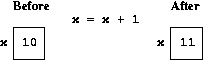
\includegraphics[width=5cm]{pic01}
  \end{center}
}

\frame{
  \frametitle{Dodela vrednosti $_5$}
  \begin{itemize}
    \item zapravo, ovo je pojednostavljeno gledanje
    \item Python ne briše stare podatke
    \item dodela vrednosti je više kao stavljanje oznake na neku vrednost, govoreći ,,ovo je \texttt{x}``
  \end{itemize}
  \begin{center}
    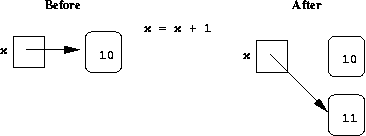
\includegraphics[width=6cm]{pic02}
  \end{center}
}

\frame{
  \frametitle{Čitanje ulaza}
  \begin{itemize}
    \item svrha \texttt{input} funkcije je da očita podatak koji unosi korisnik i smesti ga u promenljivu
    \item \texttt{<variable> = eval(raw\_input(<prompt>))}
  \end{itemize}
}

\frame{
  \frametitle{Čitanje ulaza $_2$}
  \begin{itemize}
    \item prvo se ispisuje \texttt{prompt}
    \item čeka se na korisnika da unese vrednost i pritisne enter
    \item izraz koji je unet se \texttt{eval}-uira iz niza znakova u Python vrednost (broj)
    \item taj broj se dodeljuje promenljivoj
  \end{itemize}
}

\frame{
  \frametitle{Višestruka dodela}
  \begin{itemize}
    \item više vrednosti se može izračunati istovremeno
    \item \texttt{<var>, <var>, ... = <expr>, <expr>, ...}
    \item izračunaj izraze na desnoj strani i dodeli ih promenljivama na levoj strani
  \end{itemize}
}

\frame{
  \frametitle{Višestruka dodela $_2$}
  \begin{itemize}
    \item \texttt{zbir, razlika = x+y, x-y}
    \item kako možemo zameniti vrednosti promenljivama \texttt{x} i \texttt{y}?
    \begin{itemize}
      \item zašto ovo ne radi? \\
        \texttt{x = y} \\
        \texttt{y = x}
    \end{itemize}
    \item možemo upotrebiti treću (pomoćnu) promenljivu
  \end{itemize}
}

\begin{frame}[fragile]
  \frametitle{Višestruka dodela $_3$}
  \begin{itemize}
    \item zamena vrednosti pomoću višestruke dodele je jednostavna u Pythonu: \\
      \texttt{x,y = y,x}
  \end{itemize}
\begin{minted}[linenos=false]{python}
>>> x = 3
>>> y = 4
>>> print x, y
3 4
>>> x, y = y, x
>>> print x, y
4 3
\end{minted}
\end{frame}

\begin{frame}[fragile]
  \frametitle{Višestruka dodela $_4$}
  \begin{itemize}
    \item možemo koristiti istu ideju za unos više promenljivih pomoću jednog \texttt{input}-a
    \item vrednosti koje unosimo razdvajamo zarezom
  \end{itemize}
\begin{minted}[linenos=false]{python}
def babezabe():
    babe, zabe = eval(raw_input('Unesite broj baba i broj žaba: ')
    print('Naručili ste', babe, 'baba i', zabe, 'žaba.')

>>> babezabe()
Unesite broj baba i žaba: 3, 2
Naručili ste 3 baba i 2 žaba.
\end{minted}
\end{frame}

\frame{
  \frametitle{Konačna petlja}
  \begin{itemize}
    \item \myblue{konačna petlja} izvršava svoje \myblue{telo} određeni broj puta
    \item kada petlja počne zna se tačno koliko će \myblue{iteracija} biti
    \item \texttt{for <var> in <sequence>:}\\ 
      \texttt{\ \ <body>}
    \item telo petlje se određuje uvlačenjem redova teksta u programu
  \end{itemize}
}

\begin{frame}[fragile]
  \frametitle{Konačna petlja $_2$}
\begin{minted}[linenos=false]{python}
for <var> in <sequence>:
  <body>
\end{minted}
\begin{itemize}
  \item promenljiva \texttt{var} zove se \myblue{indeks petlje}
  \item u svakom prolazu petlje uzima narednu vrednost iz date sekvence
\end{itemize}
\end{frame}

\begin{frame}[fragile,shrink=10]
  \frametitle{Konačna petlja $_3$}
\begin{minted}[linenos=false]{python}
>>> for i in [0,1,2,3]:
      print (i)

0
1
2
3
>>> for odd in [1, 3, 5, 7]:
      print(odd*odd)

1
9
25
49
>>>
\end{minted}
\end{frame}

\frame{
  \frametitle{Konačna petlja $_4$}
  \begin{itemize}
    \item u \texttt{chaos.py} šta predstavlja \texttt{range(10)}? \\
      \texttt{>}\texttt{>}\texttt{> range(10)} \\
      \texttt{(0,1,2,3,4,5,6,7,8,9)} \\
      \texttt{>}\texttt{>}\texttt{> list(range(10))} \\
      \texttt{[0,1,2,3,4,5,6,7,8,9]}
    \item \texttt{range} je Python funkcija koja generiše niz brojeva počevši od 0
    \item \texttt{list} je Python funkcija koja sekvencu konvertuje u listu
    \item telo petlje se izvršava 10 puta (ima 10 elemenata u sekvenci)
  \end{itemize}
}

\frame{
  \frametitle{Konačna petlja $_5$}
  \begin{itemize}
    \item \texttt{for} petlja menja tok izvršavanja programa
    \item predstavlja deo struktura za \myblue{kontrolu toka programa}
  \end{itemize}
  \begin{center}
    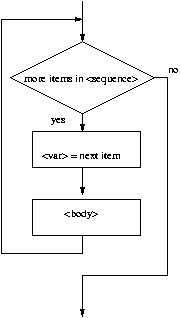
\includegraphics[width=3cm]{pic03}
  \end{center}
}

\section{Primer 2}

\frame{
  \frametitle{Primer programa: obračun kamata}
  \begin{itemize}
    \item analiza
    \begin{itemize}
      \item novac položen na račun u banci donosi kamatu
      \item koliko će biti novca na računu za 10 godina?
      \item ulazi: početno stanje, kamata
      \item izlaz: stanje na računu za 10 godina
    \end{itemize}
  \end{itemize}
}

\frame{
  \frametitle{Primer programa: obračun kamata $_2$}
  \begin{itemize}
    \item specifikacija
    \begin{itemize}
      \item ulazi: \\
        \texttt{principal} -- početno stanje na računu \\
        \texttt{apr} -- godišnja kamata izražena kao decimalni broj
      \item izlaz: stanje na računu za 10 godina
      \item veza: stanje na računu posle jedne godine iznosi \texttt{principal*(1+apr)}; ovo treba izračunati 10 puta
    \end{itemize}
  \end{itemize}
}

\frame{
  \frametitle{Primer programa: obračun kamata $_3$}
  \begin{itemize}
    \item dizajn
    \begin{itemize}
      \item ispiši uvodnu poruku
      \item unesi početno stanje računa (\texttt{principal})
      \item unesi godišnju kamatu (\texttt{apr})
      \item ponavljaj 10 puta: \texttt{pricipal = principal*(1+apr)}
      \item ispiši stanje računa
    \end{itemize}
  \end{itemize}
}

\frame{
  \frametitle{Primer programa: obračun kamata $_4$}
  \begin{itemize}
    \item implementacija
    \begin{itemize}
      \item svaki red specifikacije se preslikava na jedan red u Pythonu (u ovom primeru!)
      \item ispiši uvodnu poruku \\
        \texttt{print('Vrednost 10-godišnjeg ulaganja.')}
      \item unesi početno stanje računa \\
        \texttt{principal = eval(raw\_input('Početni ulog: '))}
      \item unesi godišnju kamatu \\
        \texttt{principal = eval(raw\_input('Unesite kamatu: '))}
      \item ponavljaj 10 puta \\
        \texttt{for i in range(10):}
      \item izračunaj principal \\
        \texttt{principal = principal*(1+apr)}
      \item ispiši vrednost principal-a nakon 10 godina \\
        \texttt{print('Vrednost iznosi:', principal)}
    \end{itemize}
  \end{itemize}
}

\begin{frame}[fragile]
  \frametitle{Primer programa: obračun kamata $_5$}
\begin{minted}[linenos=false]{python}
# futval.py
# Program racuna vrednost investicije
# 10 godina nakon ulaganja

print("Vrednost 10-godišnjeg ulaganja.")
principal = eval(raw_input("Početni ulog: "))
apr = eval(raw_input("Unesite kamatu: "))
for i in range(10):
    principal = principal * (1 + apr)
print ("Vrednost iznosi:", principal)
\end{minted}
\end{frame}

\begin{frame}[fragile]
  \frametitle{Primer programa: obračun kamata $_6$}
\begin{verbatim}
$ python futval.py
Vrednost 10-godisnjeg ulaganja.
Unesite pocetni ulog: 100
Unesite kamatu: .03
Vrednost iznosi: 134.391637934
$ python futval.py
Vrednost 10-godisnjeg ulaganja.
Unesite pocetni ulog: 100
Unesite kamatu: .1
Vrednost iznosi: 259.37424601
\end{verbatim}
\end{frame}

\end{document}